\documentclass[letterpaper,12pt]{article}
\usepackage[margin=1in]{geometry}
\usepackage{setspace}
\usepackage{graphicx}
\usepackage{url}
\usepackage{wrapfig}



\begin{document}

\begin{center}
    \par{\bf \LARGE Synthotron}
    \par{\bf \large Live Music Performance with Android}
    \par{\large 18-551 Spring 2014 Capstone Project}
    \par{\large Michael Nye (mnye), Michael Ryan (mer1)}
\end{center}



\section{The Problem}

Music performance applications on Android are virtually non-existent. Part of this problem is that historically, Android has had audio latency that is too large to facilitate responsive live performance. Latency also varies wildly between devices and OS versions. Some devices enjoy latency around 100-150ms, while others have something closer to 300-350ms. This is not yet low enough for a traditional keyboard interface, but it allows for performance on an appropriate interface with CD-quality audio (44.1kHz, 16-bit samples) in real-time.



\section{The Solution}
Synthotron addresses the need for a real-time music performance and synthesis application on the Android platform. We avoid the usual pitfalls of long latency times by scheduling music instead of playing it as a response to user touch input. This allows the application to compensate for latency and provide synchronized visual and audio feedback to users. The interface lets users create individual measures by the sixteenth notes and string eight measures together in the sequencer. The sequenced track can also loop to allow users to compose or perform with a backing track.

Synthotron also presents a satisfying range of audio synthesis options. The subtractive synthesizer, FM synthesizer, and drum machine each have their own private effects as well as shared mastering effects. These include reverb, vibrato and tremolo LFOs, a ring modulator, and three-band EQ. These effects are important for users to feel like they are interacting with a full-featured synthesizer and vastly increase the range of tones and music that one can create.



\section{Architecture}

Synthotron is designed in two connected layers: a Java frontend, and a C++ backend built using the Android NDK. The frontend is responsible for user interface and scheduling notes, while the backend is responsible for generating and processing the audio signal. The two layers communicate using a MIDI style protocol.

\subsection{Frontend}

The frontend provides a user interface for creating and scheduling one measure loops. For more details on the interface, see Section \ref{sec:interface}.

The interface code communicates with a timing manager. \textbf{TODO: DESCRIBE THIS}


\subsection{Backend}

The backend spawns into a separate thread and continuously generates audio output, feeding it to the audio driver for playback. In order to trigger notes or change effect parameters, a Java interface is provided to pass MIDI messages to the backend.

The backend is an adaptation of an audio processing framework developed by Michael Nye called ClickTrack\cite{clicktrack}. ClickTrack provides a generic interface for modular processing blocks. These blocks can be one of:
\begin{enumerate}
    \item Producer, which produces audio on its own (e.g.\ oscillators)
    \item Consumer, which takes audio input and passes them to outside sources (e.g.\ speakers)
    \item Filter, which takes in audio and produces new audio output (e.g.\ reverb)
\end{enumerate}
These blocks are connected using channels which contain circular buffers. Blocks have support for an arbitrary number of input channels and an arbitrary number of output channels. This allows for modularity of components, and makes complicated topologies simple to implement.

When requested to handle the next buffer, an audio consumer ask their input channels for audio. The channel either has the requested audio and provides it right away, or asks its parent generator to produce the audio and push it to the buffer. This allows all audio timing to be managed by a single end point and lazily generate audio as needed to maintain seamless playback.

Our project makes heavy use of this modularity and composability; the final project contains 38 separate processing blocks. The majority of these processing blocks were implemented for this project.



\section{Interface}
\label{sec:interface}

\subsection{Piano Roll}
The piano roll is a common interface for computer synthesizers. It  presents the keys of a piano with note name labels on the vertical axis and outlines a grid on which the user can place notes that follow time on the horizontal axis.

\begin{figure}[h]
\centering
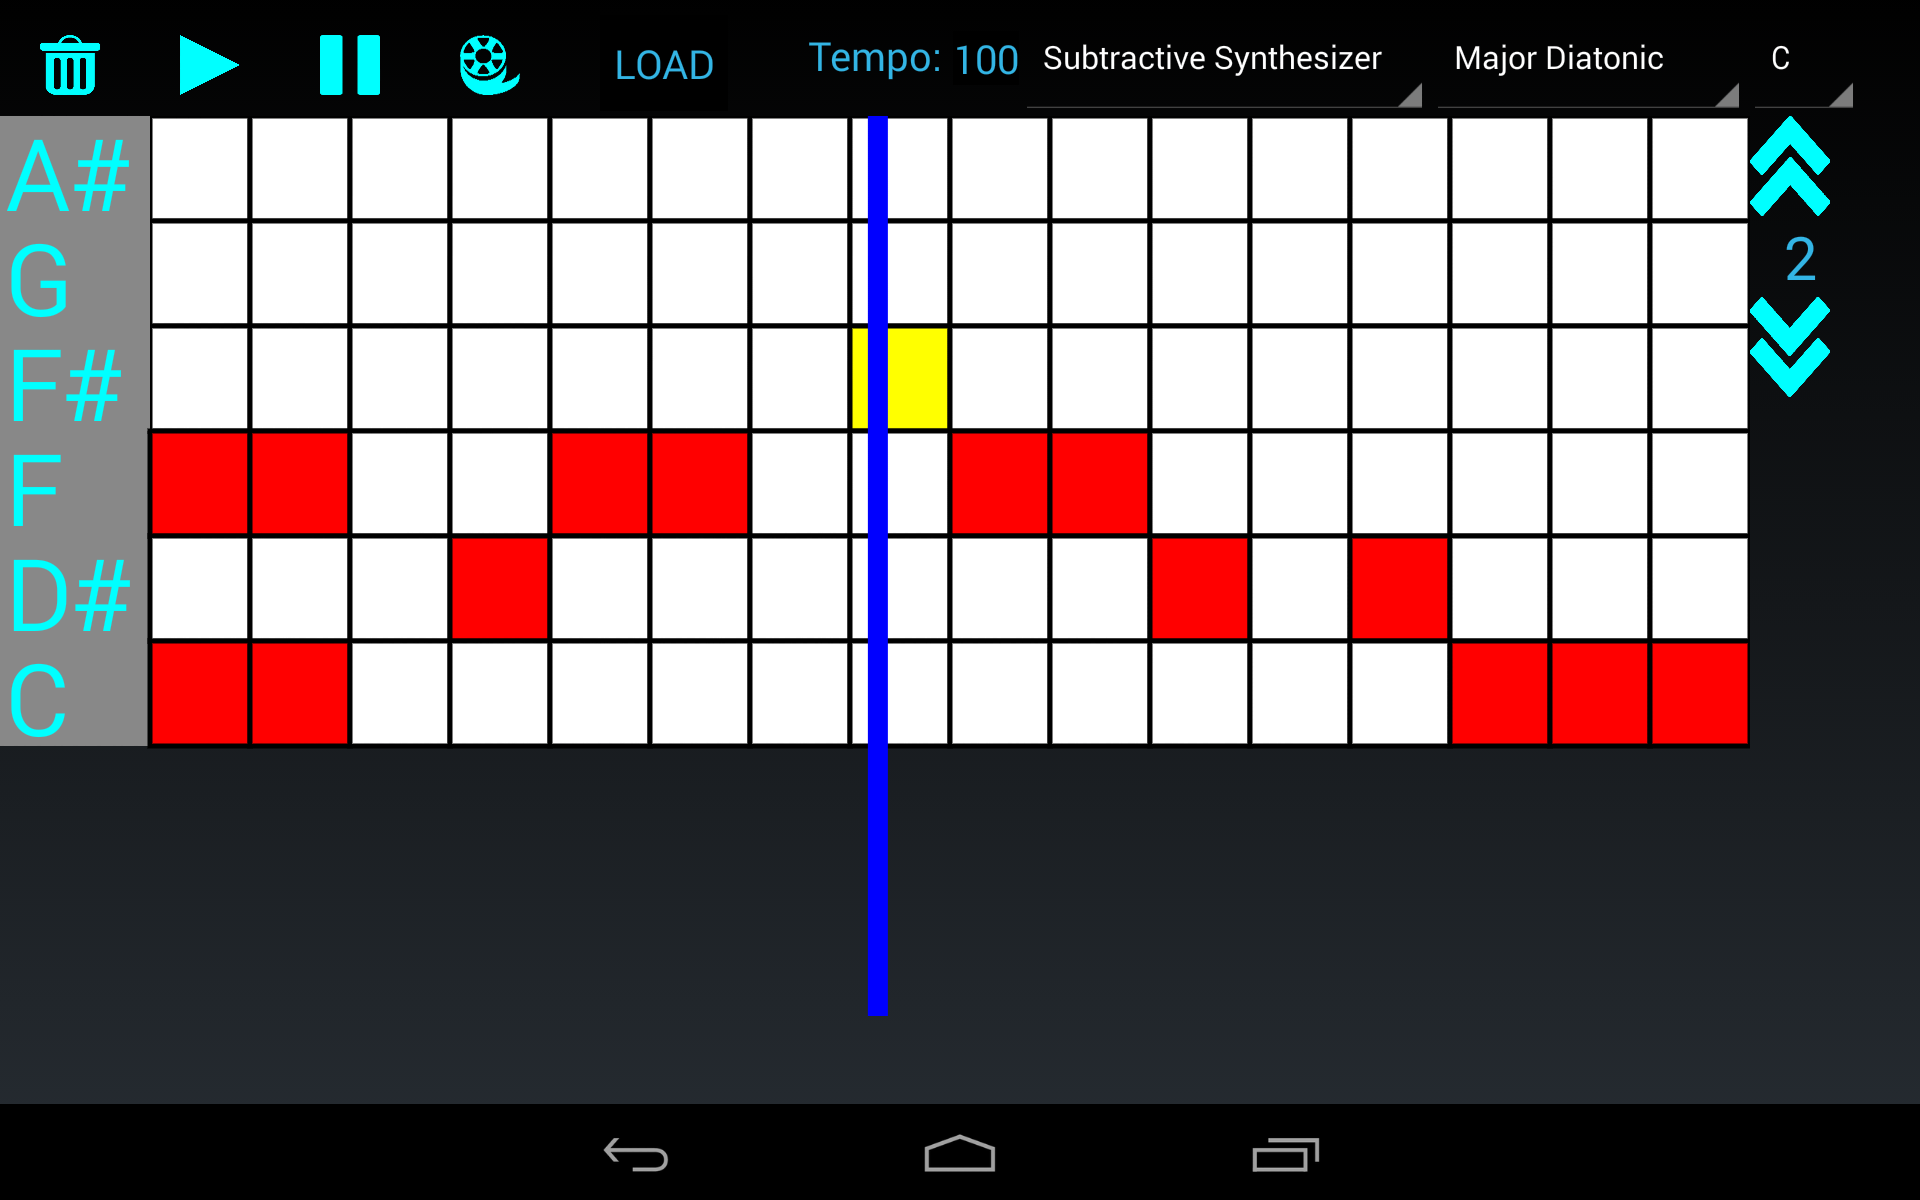
\includegraphics[width=0.4\textwidth]{figures/pianoroll.png}
\caption{Piano Roll interface}
\label{fig:pianoroll}
\end{figure}

Our piano roll has been simplified to limit the user to a specific key. In most cases, this is not only sufficient, but makes composition easier. The user can choose between diatonic, pentatonic, and blues major and minor scales. Restricting notes to one key helps inexperienced composers generate satisfying music with only a few touches of the screen. 

\subsection{Sequencer}

Just as the piano roll composes notes on a grid of quarter beats, the seqeuncer composes measures. The vertical axis is now occupied by Synthotron's three channels. Users can copy measures from one cell to another and save or load individual measures and whole songs.

\begin{figure}[h]
\centering
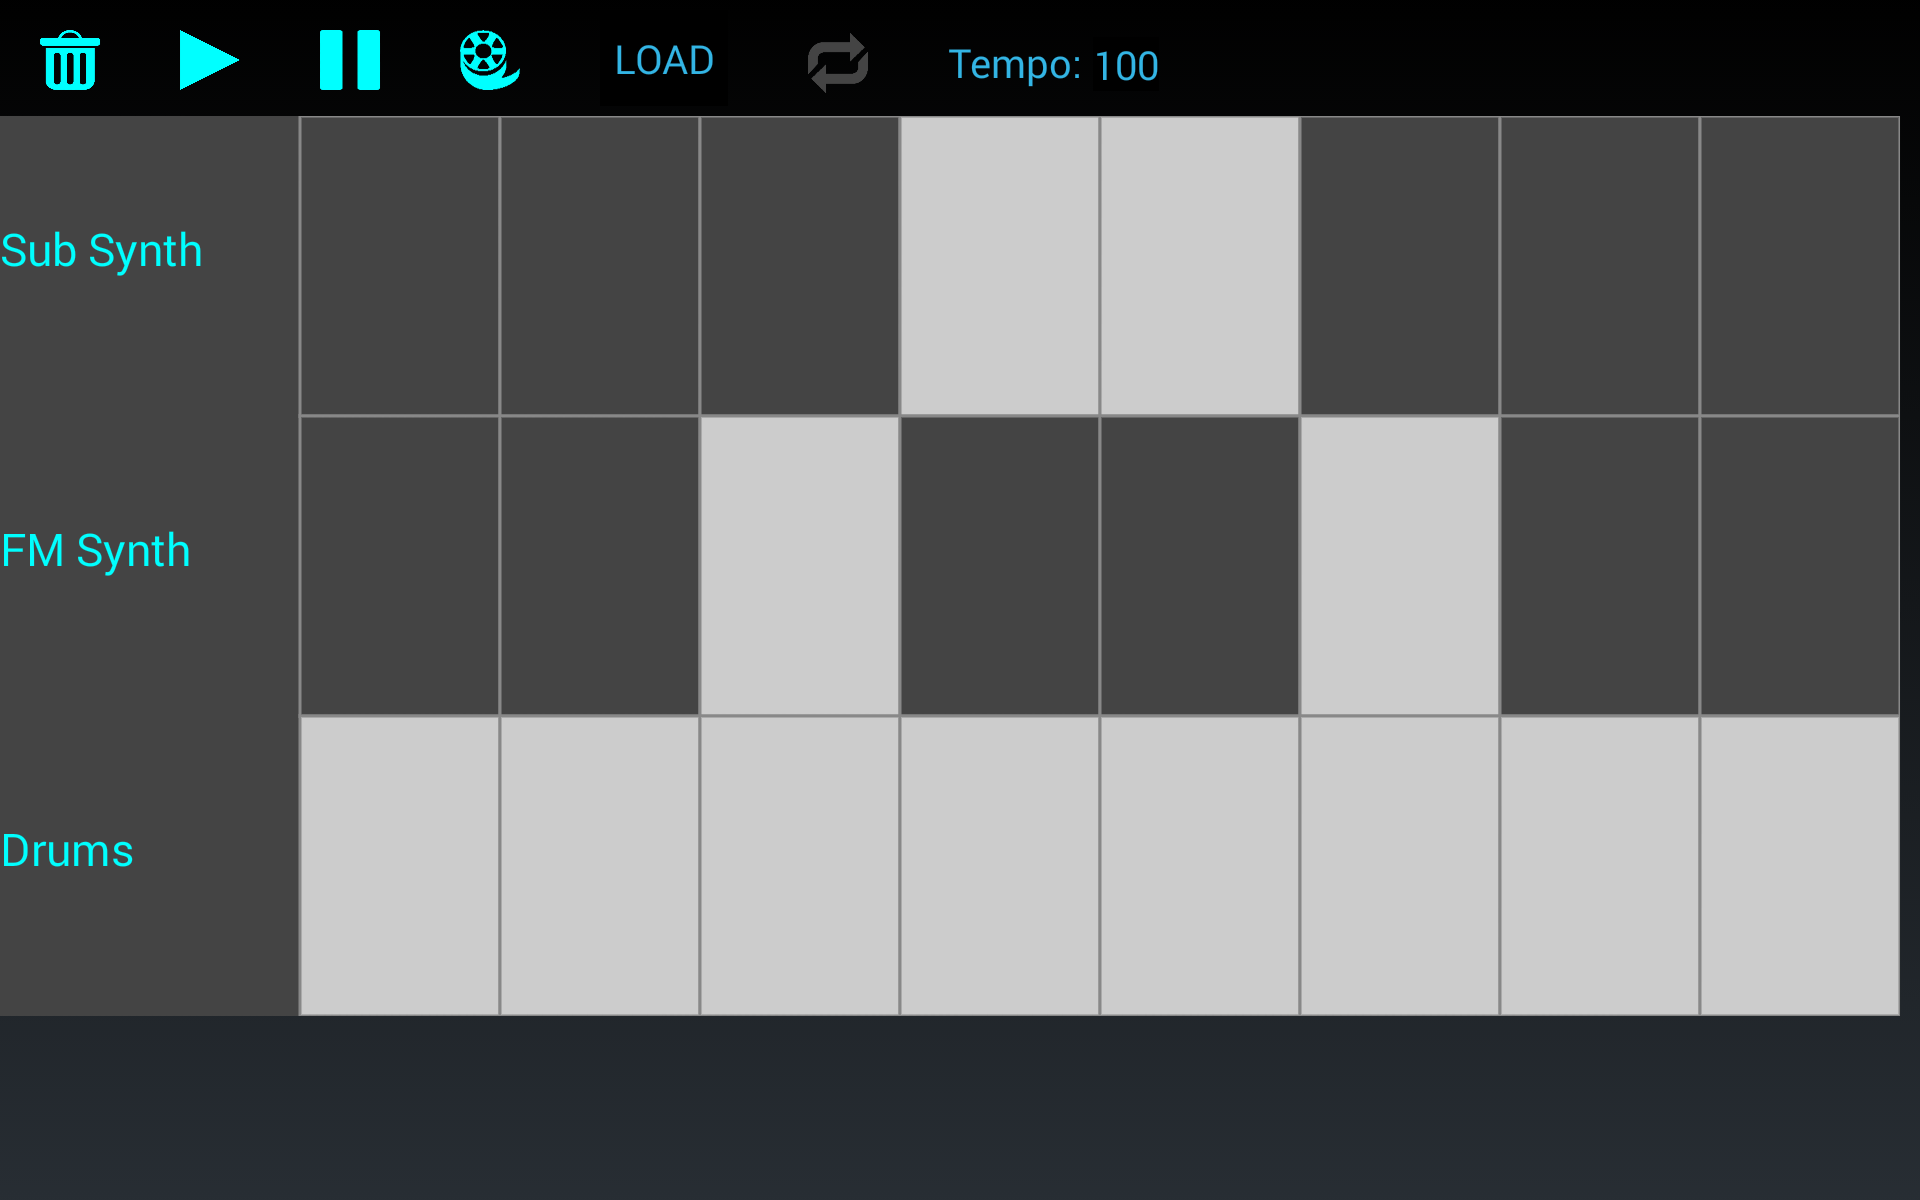
\includegraphics[width=0.4\textwidth]{figures/sequencer.png}
\caption{Sequencer interface}
\label{fig:sequencer}
\end{figure}

\subsection{Synthesizer and Mastering}

\begin{wrapfigure}{r}{0.5\textwidth}
\centering
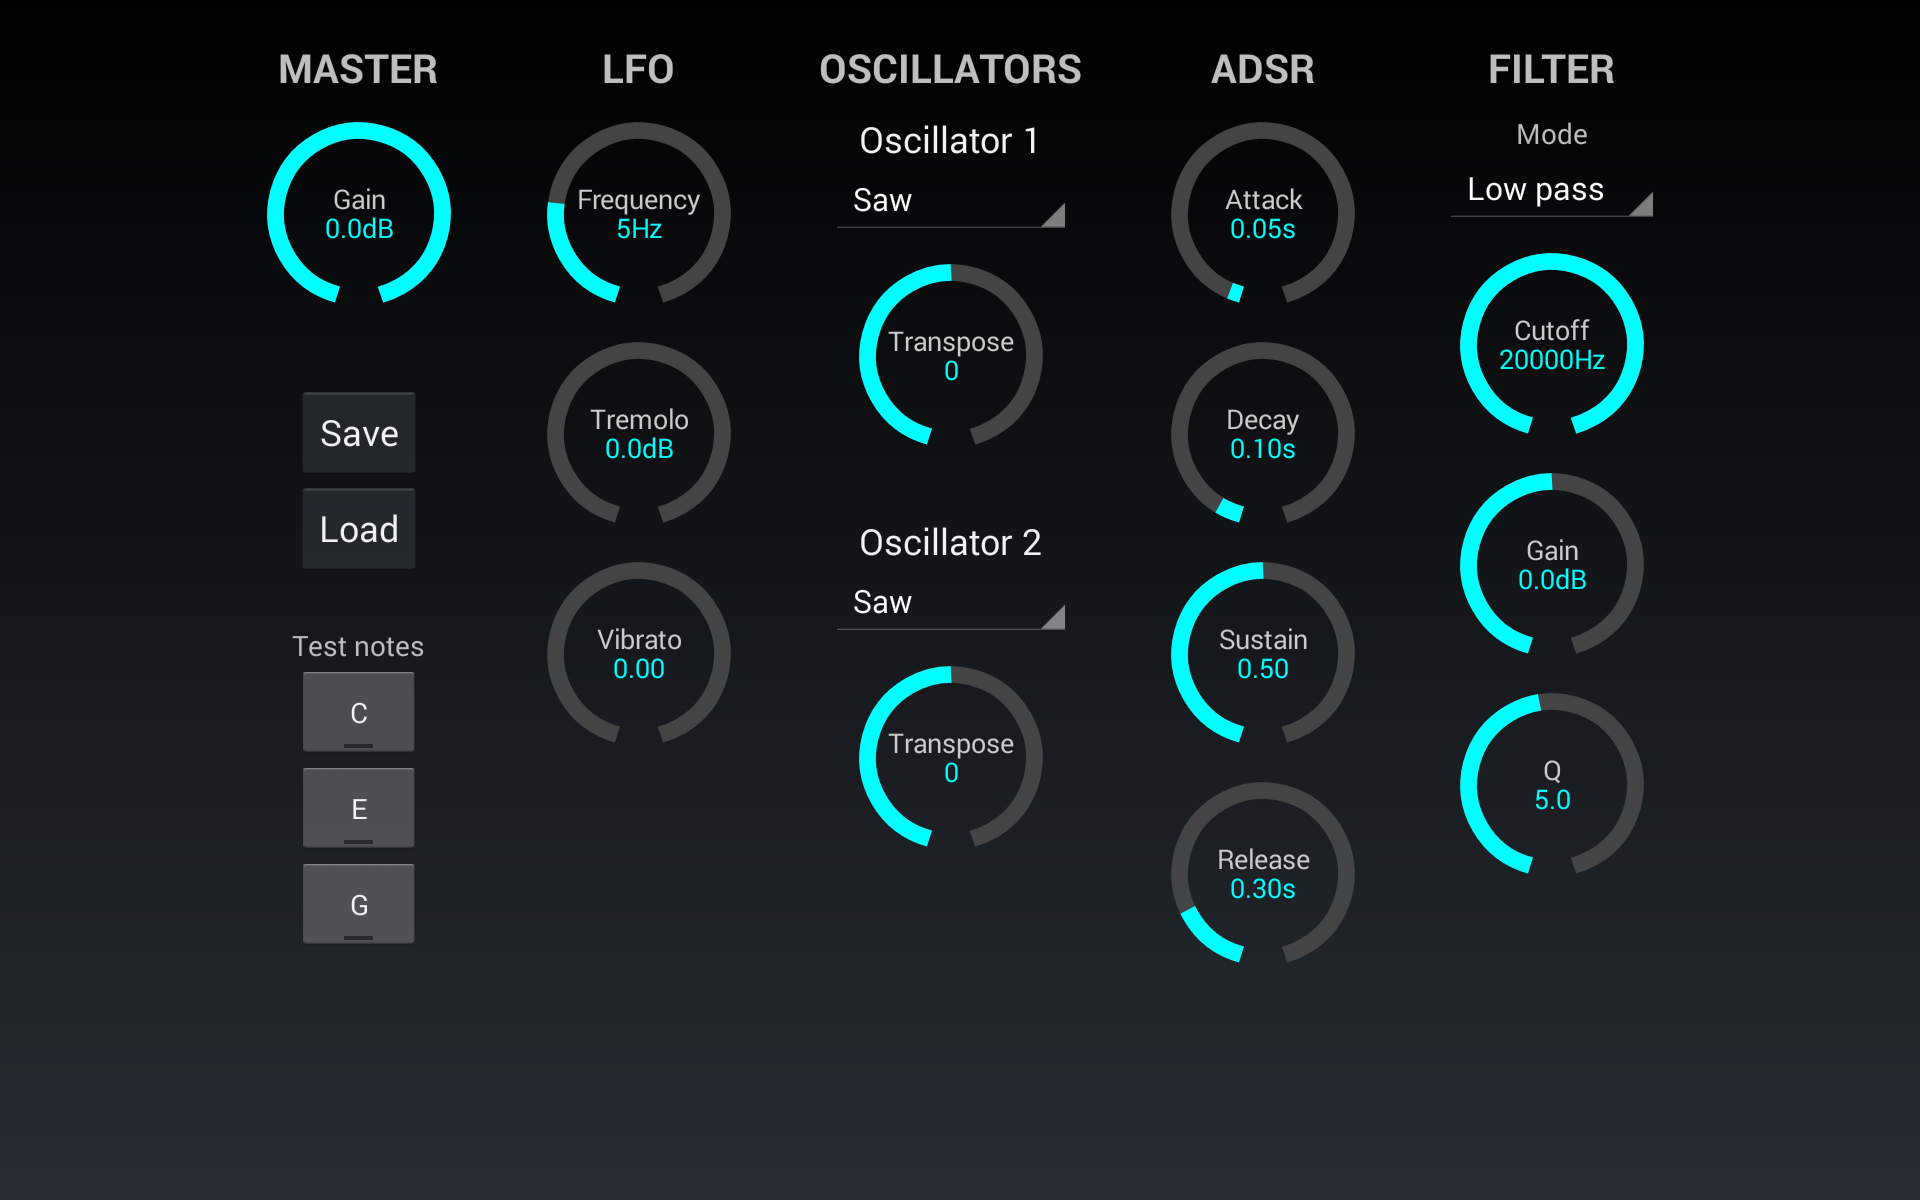
\includegraphics[width=0.4\textwidth]{figures/subtractivesynth.png}
\caption{Subtractive Synthesizer}
\label{fig:subtractivesynth}
\end{wrapfigure}

The synthesizer and mastering interfaces feature a number of knobs to control the aspects of each instrument and the entire synthesis engine. The knobs act like analog knobs on a physical synthesizer, and this feeling is important for providing a satisfying experience when controlling Synthotron.

Synthesizer control panels also allow for the saving and loading of favorite configurations.

\section{Audio Processing Algorithms}

\subsection{Oscillators}

The most basic element of synthesis is the oscillator. An oscillator is a device that simply emits a certain waveform at an adjustable frequency. Our oscillators are designed to emit the set of fundamental waveforms: sine waves, saw waves, square waves, triangle waves, and pulse waves. These waveforms are desirable for music applications because they have rich upper harmonics, which gives lots of flexibility to carve different tonalities out of them.

\begin{wrapfigure}{r}{0.5\textwidth}
\centering
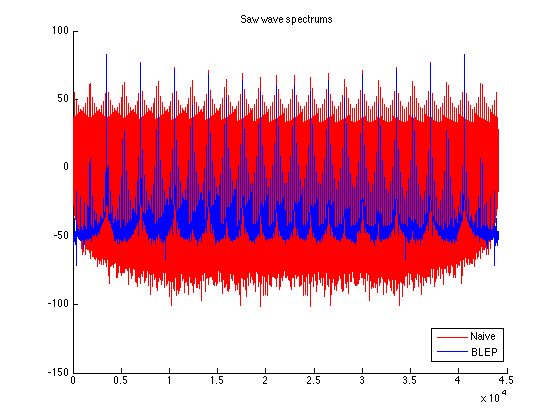
\includegraphics[width=0.4\textwidth]{figures/blep-spectrum.png}
\caption{Frequency content of saw wave}
\label{fig:polyblep-spectrum}
\end{wrapfigure}

Implementing these waveforms in the naive way (i.e.\ with sharp edges at transition points) implicitly decimates a waveform with arbitrarily high frequency content. The result is a waveform that has large amounts of aliasing; this is especially evident when playing high frequency notes.


In order to avoid this problem, our oscillators use a method called \textbf{Polynomial Bandlimited Steps}, or PolyBLEP\cite{polyblep}. PolyBLEP works by rounding the edges around a sharp transition point using a polynomial. If \texttt{t} represents the phase of our waveform normalized between 0 and 1, and \texttt{dt} represents the change in our phase each sample, then the PolyBLEP term can be computed as follows:

\begin{verbatim}
if (t < dt) {
    t /= dt;
    return t+t - t*t - 1.0;
} else if (t > 1.0 - dt) {
    t = (t - 1.0) / dt;
    return t*t + t+t + 1.0;
} else {
    return 0.0;
}
\end{verbatim}

This method is incredibly effective, and can pull down the peak sidelobe aliasing my 50 to 100 decibels for a saw wave. See Figure \ref{fig:polyblep-spectrum} for a comparison of the frequency content of a naive saw wave, and a PolyBLEP saw wave.


\subsection{Low Frequency Oscillators}

A typical oscillator is used to generate an audible waveform. Low Frequency Oscillators, or LFOs, are oscillators at sub-audible frequencies that are instead used to modify parameters of filters or other oscillators. Our application uses LFOs to create two different effects: vibrato, and tremolo.

Vibrato uses an LFO to modify the frequency a waveform oscillates at. For example, we can use the following equation to compute the instantaneous frequency of an oscillator from its stationary frequency as $f_i = f_s \cdot 2^{LFO(t) \cdot I}$, where $LFO(t)$ represents the LFO waveform, and $I$ controls the depth of the vibrato, where 0 represents no vibrato, and 1 represents an octave.

Tremolo uses an LFO to modify the gain of an input signal to create a wavering sound. The tremolo gain can be computed as $10^{LFO(t) \cdot I}$, where $LFO(t)$ represents the LFO waveform, and $I$ controls the depth of the tremolo.


\subsection{ADSR Envelopes}

\begin{wrapfigure}{r}{0.5\textwidth}
\centering
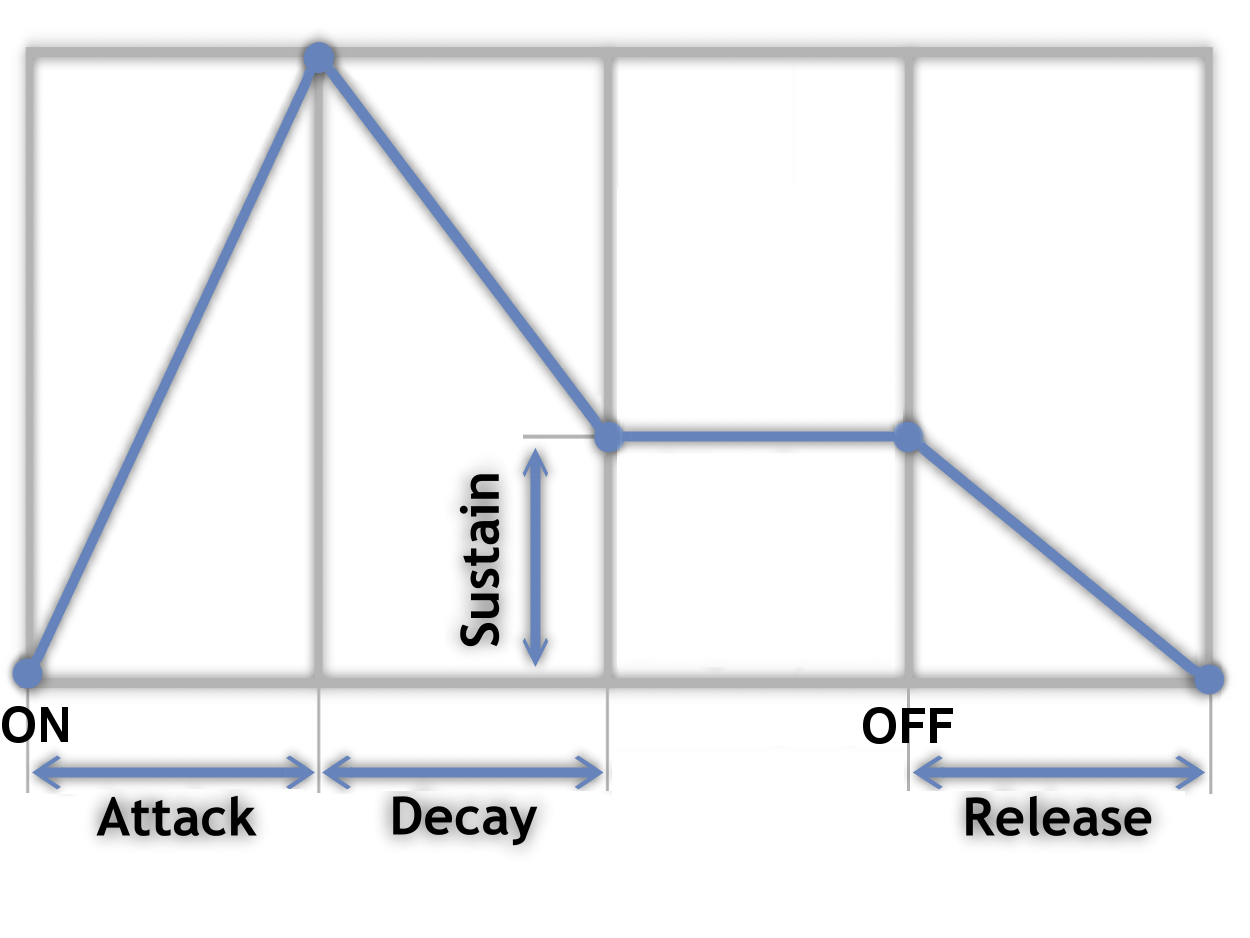
\includegraphics[width=0.4\textwidth]{figures/adsr.png}
\caption{ADSR Envelopes}
\label{fig:adsr}
\end{wrapfigure}

ADSR Envelopes (short for Attack, Decay, Sustain, Release) are used to shape a note when it is trigged. A note passes through four states: the attack, decay, sustain, and release state. Attack, decay and release occur for a fixed increment of time, while the sustain state can last indefinitely.

In the attack state, the gain of the note scales from 0 to 1; this gives the note a fade in. In the decay state, the gain scales back from 1 to the sustain level; this backs the note off and makes the attack sound sharper. During the sustain state, the gain remains constant until the note is told to stop. It finally enters the release state, where the gain scales from the sustain level back to zero.


\subsection{Compressors and Limiters}

\begin{wrapfigure}{r}{0.5\textwidth}
\centering
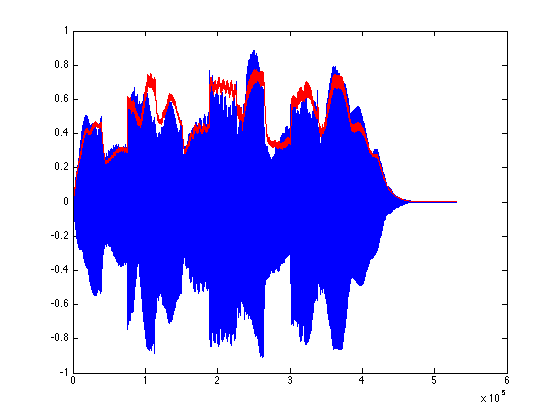
\includegraphics[width=0.45\textwidth]{figures/envelope-fit.png}
\caption{Envelopes Fitting}
\label{fig:envelopes}
\end{wrapfigure}

Compressors and limiters are a class of nonlinear processors that respond to the signal level of its inputs. The devices first rely on an envelope estimation, that determines the amplitude of the signal.

In order to estimate the envelope of a signal, we rely on leaky integration of our signal. This takes the from $env(t) = \alpha \cdot env(t-1) + (1-\alpha) \cdot x(t)$. However, in order to rise quickly and fall slowly, we use to different values of $\alpha$. A small value of $\alpha$ is used if $x(t) > env(t-1)$, and a larger value is used if $x(t) < env(t-1)$. A sample envelope estimation is show in Figure \ref{fig:envelopes}.

Once we have an envelope function, a limiter and compressor can use to calculate a new gain. Both devices have a set threshold; in Figure \ref{fig:compressor-limiter}, the threshold is set to 0.5. A limiter scales back a signal so that its output level never exceeds the threshold. A compressor scales back a signal by a certain ratio. In Figure \ref{fig:compressor-limiter}, this ratio is set to 0.5, so it reduces the signal by half the value it exceeds the threshold.

\begin{figure}[h]
\centering
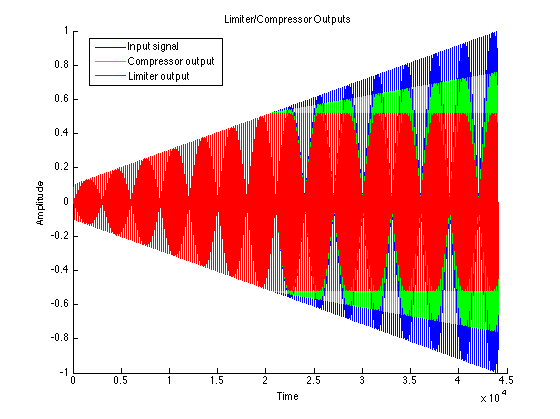
\includegraphics[width=0.8\textwidth]{figures/limiter-compressor-output.png}
\caption{Compressor and limiter outputs}
\label{fig:compressor-limiter}
\end{figure}


\subsection{Reverberator}

A reverberator is used to simulate the echoing of a room, in effect placing a synthesized signal in a real space. How to simulate this effect is still a widely discussed topic. For this project, we chose to implement a seminal method described by JA Moorer in the late 1970s\cite{moorer}. The Moorer reverberator takes on two stages in series.

The first stage is a tapped-delay line. This attempts to simulate the first few arrivals of a multipath propagation. The individual delays should be relatively prime, in order to accidentally create strange frequency responses. Our first stage has 17 taps, the last of which arrives about 80 milliseconds after the input signal.

The second stage is a set of parallel comb filters. The comb filter attempts to simulate the random arrival of a large number of faint multipaths, in order to make the reverberation sound more full. The gains of the comb filter can be set to change the decay time of the filter. Our second stage uses 6 comb filters with delays ranging from 50 to 80 milliseconds.


\subsection{Filters and Equalizers}

An important part of synthesis is filters that allow carving of the frequency spectrum. While in many applications, sharp filters with low sidebands are more desired, musical applications actually prefer less extreme filters. To do so, we implement first and second order filters, as described in Reference \cite{dafx}.

First order filters support low-pass and high-pass filters, with 12dB/octave roll off. Second order filters support low-pass and high-pass filters with 24dB/octave roll off, as well as shelfing and peaking filters.

A shelfing filter allows you to specify a gain below or above a certain cutoff, while maintaining 0dB gain outside the passband. A peak filter allows you to specify a gain at a certain frequency, with a roll-off set by an adjustable Q-factor, again with 0dB gain outside the passband.

By composing several of these filters in different modes, we can create multi-point equalizers.


\subsection{Ring Modulator}

A ring modulator is a very simple device. It simply multiples a signal by a fixed frequency sine wave. The resulting signal output resembles the input, but shifted in frequency space. It can be used to create interesting pitch shifts and aliasing effects, especially on instruments that aren't inherently pitched such as drums.

\section{Timing and optimization}
One of the largest challenges for developing on Android is the audio latency time. Each device has a different optimal buffer size and delay between the audio command being sent and output from speaker. In this project, we optimized for the Google Nexus 7 2013, which had a latency of XXXXXXX ms.
The piano roll and sequencer both include a moving bar to keep time with the audio track. The velocity of these bars is directly proportional to the tempo of the song. We also keep the bars moving delayed with respect to the actual scheduling of the notes with a linear offset.

\section{Live demonstration}
The demo included the free use of Synthotron with a variety of presets to showcase all functionality. Attendees toyed with all features of the system while being guided on functionality and were encouraged to loop a rock drum track while experimenting in the piano roll, the main method of live performance with the application. Completed demos included several synthesizer presets and two songs - "More Than a Feeling" by Boston and "The District Sleeps Alone" by The Postal Service.

\section{Libraries used}
\begin{itemize}
    \item OpenSLES: Industry standard embedded audio API, provided by Google as the core Android audio driver. Used to send all music to the system for playback. \cite{opensles}
    \item Guava: Google Java Collections library \cite{guava}
    \item Gson: Google Java JSON Serialization library \cite{gson}
\end{itemize}



\clearpage
\section*{Final Work Breakdown}

\onehalfspacing
\begin{tabular}{ c | l }  

  Week 1 (Feb 16 - Feb 22) & Initial proposal and presentation Feb 18 \\ 
                           & Experiment with Android audio latency Feb 22 \\ \hline
  Week 2 (Feb 23 - Mar 2)  & Nye - Begin porting ClickTrack to Android \\
                           & Ryan -  Develop barebones sequencer, piano roll, or keyboard \\ &interface on Android \\ \hline
  Week 3 (Mar 9 - Mar 15)  & Spring break!  \\ \hline
  Week 4 (Mar 16 - Mar 22) & Nye - ClickTrack functionality on Android \\ 
                           & Ryan - Combine interface with ported audio production \\ \hline
  Week 5 (Mar 23 - Mar 29) & Nye - Finish port of ClickTrack with Java interface \\
                           & Ryan - Refactor and make robust interface \\ \hline
  Week 6 (Mar 30 - Apr 5)  & \textbf{Updates} \\
                           & Begin expanding functionality for additional instruments \\ & and effects\\ \hline
  Week 7 (Apr 6 - Apr 12)  &  Nye - Additional effects, FM Synth \\
                           & Ryan - Develop sequencer interface \\ \hline
  Week 8 (Apr 13 - Apr 19) & Load/Save configurations and songs \\                           \hline
  Week 9 (Apr 20 - Apr 26) & Nye - Additional effects and cleanup of audio engine \\
                           & Ryan - Additional effects and cleanup of interface \\ \hline
  Week 10 (Apr 27 - May 3) & Completed project and working demo  \\ \hline
  Week 11 (May 4 - May 11) & Final report  \\ 
\end{tabular}
  

\clearpage
\begin{thebibliography}{9}
\singlespacing

\bibitem{caustic}
    \url{https://play.google.com/store/apps/details?id=com.singlecellsoftware.caustic}

\bibitem{clicktrack}
    \url{https://github.com/thenyeguy/ClickTrack}

\bibitem{dafx}
    lzer, Udo. ``DAFX digital audio effects.'' 2nd ed. 
    Chichester, West Sussex, England: Wiley, 2011. Print.

\bibitem{moorer}
    Moorer, James A. ``About this reverberation business.'' 
    Computer music journal (1979): 13-28.

\bibitem{opensles}
    \url{http://www.khronos.org/opensles/}

\bibitem{polyblep}
    \url{http://www.kvraudio.com/forum/viewtopic.php?t=375517}

\bibitem{guava}
    \url{http://code.google.com/p/guava-libraries/}

\bibitem{gson}
    \url{https://code.google.com/p/google-gson/}

\end{thebibliography}


\end{document}
